%% Los margenes, tipo de hoja y estilo BOOK
\documentclass[a4paper,11pt,twoside,openright,titlepage]{book}
\usepackage[a4paper,left=1in,right=1in,top=0.6in]{geometry}

\usepackage[T1]{fontenc}    %Ineterprete de tíldes
%\usepackage[Latin1]{inputenc}
\usepackage{amsmath,amssymb}    %Paquete de entornos matematicos
\usepackage{listings}
\usepackage{natbib}
\usepackage[english,spanish]{babel}
\selectlanguage{spanish} 
\usepackage{graphicx}
\usepackage{hyperref}
\usepackage{psfrag}
\usepackage{float}
\usepackage{quotchap}
\usepackage{epsfig}
\usepackage[all]{xy}
\usepackage[utf8]{inputenc}
\usepackage{epsfig}
\usepackage{makeidx}
\usepackage{xcolor}
\usepackage{ifthen}
\usepackage{multicolpar}    %Para poner texto en columnas en plan articulo intercalado con texto normal
\usepackage{multicol,multirow}

\usepackage{url}        %Para direcciones web
\usepackage{marvosym}   %Para imprimir el simbolo de \EUR euro
%\usepackage{eurosym}   %Para imprimir el simbolo de \euro euro
\usepackage{fancybox}   %Para tablas con bordes redondeados


%% Modificación de la plantilla para adaptarla a los requisitos de PFC
\usepackage{fancyhdr}
\pagestyle{fancy}
%%% Cabeceras y pies de página
\fancyhead[CE,CO]{\emph{\titulo}}
\fancyhead[LE,LO,RE,RO]{}
\fancyfoot[LE,RO]{\thepage}
\fancyfoot[CE,CO]{\leftmark}

\renewcommand{\footrulewidth}{.6pt}


\colorlet{punct}{red!60!black}
\definecolor{background}{HTML}{EEEEEE}
\definecolor{delim}{RGB}{20,105,176}
\colorlet{numb}{magenta!60!black}

\lstdefinelanguage{json}{
    basicstyle=\normalfont\ttfamily,
    numbers=left,
    numberstyle=\scriptsize,
    stepnumber=1,
    numbersep=8pt,
    showstringspaces=false,
    breaklines=true,
    frame=lines,
    backgroundcolor=\color{background},
    literate=
     *{0}{{{\color{numb}0}}}{1}
      {1}{{{\color{numb}1}}}{1}
      {2}{{{\color{numb}2}}}{1}
      {3}{{{\color{numb}3}}}{1}
      {4}{{{\color{numb}4}}}{1}
      {5}{{{\color{numb}5}}}{1}
      {6}{{{\color{numb}6}}}{1}
      {7}{{{\color{numb}7}}}{1}
      {8}{{{\color{numb}8}}}{1}
      {9}{{{\color{numb}9}}}{1}
      {:}{{{\color{punct}{:}}}}{1}
      {,}{{{\color{punct}{,}}}}{1}
      {\{}{{{\color{delim}{\{}}}}{1}
      {\}}{{{\color{delim}{\}}}}}{1}
      {[}{{{\color{delim}{[}}}}{1}
      {]}{{{\color{delim}{]}}}}{1},
}

%Definiciones de funciones para los titulos
\newlength\salto
\setlength{\salto}{3.5ex plus 1ex minus .2ex}

\newlength\resalto
\setlength{\resalto}{2.3ex plus.2ex}

\newcommand{\lsection}[1]
                {\section{#1}
                \vskip-.9\resalto   %%%% Aquí reculo el posible salto por defecto de \section
                \hrule
                \vskip+.9\salto}  %%%% vuelvo ha realizar el salto (puedes poner otra vez el 90%)


%Para imágenes de entornos estáticos \captionFigure{Texto Caption}{Texto Label}
\newcommand{\captionFigure}[2]{
    \refstepcounter{figure}
    \centerline{Figura \thefigure: #1 \label{#2}}
    \addcontentsline{lof}{section}{\thefigure.\ #1\label{#2}}
}

%Para imágenes de entornos estáticos \NOcaptionFigure{Texto Caption}{Texto Label} "No escribe el caption"
\newcommand{\NOcaptionFigure}[2]{
    \refstepcounter{figure}
    \addcontentsline{lof}{figure}{\thefigure.\ #1\label{#2}}
}


%% Datos del PFC

\newcommand{\titulo}{1718\_072\_IC \- Diseño e implementación de un hub de control domótico}
\newcommand{\autor}{Autor: Pallarés Jiménez, Ignacio}
\newcommand{\director}{Nombre Apellido1 Apellido2}
\newcommand{\tutor}{Tutor: Delgado Mohatar, Óscar}
\newcommand{\ponente}{Ponente: Anguiano Rey, Eloy}
\newcommand{\vocal}{Nombre Apellido1 Apellido2}
\newcommand{\vocalsup}{Nombre Apellido1 Apellido2}
\newcommand{\presidente}{Nombre Apellido1 Apellido2}
\newcommand{\presidentesup}{Nombre Apellido1 Apellido2}
\newcommand{\fecha}{JULIO 2018}
\newcommand{\carrera}{Grado en Ingeniería Informática}

\begin{document}
\setlength{\baselineskip}{18pt}  %% Espacio interlinea
\setlength{\parskip}{6pt plus 1pt minus 1pt} %% Espacio interpárrafo
\setlength\itemsep{6pt plus 1pt minus 1pt}
\begin{titlepage}

\begin{center}

\vspace*{2cm}

\LARGE \textsc{Universidad Autónoma de Madrid}\\

\vspace{.2cm}

\large \textsc{Escuela politécnica superior}\\

\vspace{.2cm}

\begin{figure}[h]
    \begin{center}
        \begin{minipage}[c]{0.495\linewidth}
            \rightline{\epsfig{figure=images/logo_eps.eps,width=0.5\linewidth}}
        \end{minipage}
        \begin{minipage}[c]{0.495\linewidth}
            \leftline{\epsfig{figure=images/logo_uam.eps,width=0.5\linewidth}}
        \end{minipage}
    \end{center}
    \label{fig:Escudos}
\end{figure}

\Huge \carrera\\

\vspace{1cm}

\Huge \textsc{Trabajo Fin de Grado}\\

\vspace{1.5cm}

\Huge \MakeUppercase{\textbf{\titulo}}

\vspace{3cm}


\Large \autor\\
\Large \tutor\\
\Large \ponente\\

\vspace{0.5cm}

\Large \fecha

\end{center}

\end{titlepage}

\normalsize


\newpage \thispagestyle{empty} % Página vacía


\frontmatter %Define el cuerpo inicial del libro en numeración con letras romanas

\chapter*{}

\vspace*{0.2cm}

\begin{center}

\Huge \MakeUppercase{\textbf{\titulo}}

\vspace{7cm}

\Large \autor \\
\Large \tutor \\
\Large \ponente \\

\vspace{5cm}


Grupo de la EPS (opcional) \\
Dpto. de XXXXX \\
Escuela Politécnica Superior \\
Universidad Autónoma de Madrid \\
\fecha

\end{center}

\normalsize

\newpage \thispagestyle{empty} % Página vacía


\chapter*{Resumen}

\section*{Resumen}

La domótica consiste en la automatización del hogar. Los sistemas domóticos, son aquellos capaces de domotizar una vivienda; proporcionan servicios de comunicación,
seguridad, eficiencia energética...etc. Sin duda alguna, la comunicación entre estos sistemas es algo esencial, existiendo redes cableadas e inalámbricas para ello, pudiendo
ser controlados estos sistemas desde dentro y fuera del hogar.

BRIMO es un proyecto de código abierto para la gestión y el control de dispositivos domóticos en el hogar. Es una alternativa open source de bajo coste para todas
aquellas personas que deseen domotizar su hogar de una manera barata y sencilla. No utiliza protocolos privados, y cualquiera que lo desee puede utilizar y modificar
la aplicación a su gusto.

Además, cualquier persona puede crear sus dispositivos (sensores, actuadores o cámaras) de manera sencilla, siempre que éstos sigan los requisitos establecidos.
Brimo nos ayuda, gracias a una interfaz sencilla e intuitiva, a ordenar nuestros dispositivos, visualizar sus estados y mandar comandos a los dispositivos que los acepten.

La aplicación está pensada para ejecutarse en entornos ligeros, concretamente en una Raspberry Pi 3 (precio asqequible), pero también puede ser ejecutada en cualquier ordenador tras una simple configuración.
Utiliza una arquitectura REST sobre el protocolo HTTPS para comunicarse con los dispositivos.

La función principal de Brimo es de "bridge", punto común entre el usuario y los dispositivos, se encarga de poner en contacto al usuario con los dispositivos.
\section*{Palabras Clave}
Domótica, código abierto, REST, raspberry, HTTP, sensores, MVC, actuadores, bridge.
\newpage

%-------------------------------------------------------------------------------------------------------------------------------------

\section*{Abstract}
Domotic consists of home automation. Domotic systems are those capable of automating a home; providing communication services,
security, energy efficiency ... etc. Communication between these systems is essential, existing wired and wireless networks for it,
that allows us to controll them from inside and outside the home.

BRIMO is an open-source project for the management and control of domotic devices in the home. It is a low-cost open source alternative for all people
 who want to domotize their home in a cheap and simple way. It does not use private protocols, and anyone can use or modify the application on its preferences.

Besides, anyone is able to create its own devices (sensors, actuators or cameras) in a simple way, following the application requirements. Brimo helps us, thanks to
a simple and intuitive interface, to arrange our devices, seeing their status and to send them commands.

The application is designed to be runned on lightweight devices, specifically into a Raspberry Pi 3 (low cost), but it could be also runned on any computer after a simple
configuration. It uses REST architecture over HTTPS protocol to communicate with devices.

The main function of Brimo is to act as bridge, the common point between users and devices: Brimo is the responsible of the communication between them.
\section*{Key words}

Domotic, open-source, low cost, REST, raspberry, HTTP, sensors, MVC, actuators.

\chapter*{Agradecimientos}


\tableofcontents

\newpage \thispagestyle{empty} % Página vacía

\addcontentsline{toc}{chapter}{Índice de Figuras}    %Para que aparezca en el índice
\renewcommand{\listfigurename}{Índice de Figuras} 
\listoffigures

\newpage \thispagestyle{empty} % Página vacía

\addcontentsline{toc}{chapter}{Índice de Tablas}    %Para que aparezca en el índice
\renewcommand{\listtablename}{Índice de Tablas} 
\listoftables

\newpage \thispagestyle{empty} % Página vacía

\mainmatter %Define el cuerpo principal del libro numeración normal.

% \input{preambulo}

\chapter{Introducción} 
\label{chap:intro}

\vspace{-0.2cm}

\lsection{Motivación del proyecto}

Los sistemas domóticos por lo general utilizan una arquitectura centralizada: un controlador (bridge) es el encargado de enviar y recibir información de los dispositivos domóticos y las interfaces.
 Se utilizan sistemas centralizados debido a que abaratan mucho el coste de los dispositivos domóticos, así los dispositivos tienen poca electrónica y programación, y la responsabilidad principal
 reside en el bridge. Este enfoque tiene sentido cuando se trata de muchos dispositivos en un hogar, que es el caso ideal, si solo tuviésemos un sensor carecería de sentido tener un sensor y un bridge para manejarlo.

El problema principal que existe con los sistemas centralizados se encuentra en la \textbf{compatibilidad} entre dispositivos y bridges.
Por lo que he observado~\cite{article:EstadoDelArte}, todavía falta mucha estandarización en el
ámbito de la domótica: cada fabricante usa sus medios y protocolos haciendo incompatibles bridges y dispositivos. Además, estos dispositivos no suelen ser 
muy asequibles. Por lo tanto, nos encontramos ante la necesidad de comprar todos los dispositivos de una misma marca o tener muchos bridges, lo que nos obligaría a manejar cada
dispositivo desde su correspondiente bridge.

La domótica puede hacernos la vida en el hogar mucho más sencilla, ayudándonos a ahorrar tiempo y dinero que podremos invertir en otras cosas. Los hogares todavía están muy poco automatizados, y mi principal motivación ha sido acercar la domótica 
a las personas y aprender acerca de ella. Gracias a nuestro sistema manejamos todos los dispositvos a través de un solo bridge de manera sencilla y eficaz.

\newpage
\lsection{Objetivos y enfoque}

El objetivo último de nuestro proyecto es desarrollar un sistema que sea capaz de recibir y enviar información de dispositivos domóticos y sea capaz de interactuar con el cliente. 

Los \textbf{requisitos} que debe cumplir nuestro sistema son:
\begin{itemize}
  \item \underline{Ligero.} Un bridge no debería necesitar demasiada capacidad de procesamiento y de memoria, y es necesario que no sea muy costoso, por lo tanto, la ligereza es requisito indispensable.
  \item \underline{Compatibilidad.} Necesitamos que nuestro bridge no sea únicamente compatible con un tipo de sensor, o un modelo de cámara
  \item \underline{Interfaz sencilla y adaptable a cualquier dispositivo.} Necesitamos que la interfaz de nuestro bridge sea compatible con cualquier dispositivo sin perder funcinalidad.
  \item \underline{Seguridad.} La seguridad en la domótica es algo indispensable, confío en que el día de mañana incluso las cerraduras de nuestras casas serán automáticas, y no podemos dejar la responsabilidad de la seguridad
  de nuestra a casa a un sistema con vulnerabilidades de seguridad.
  \item \underline{Escalable.} Nuestro sistema ha de ser escalable y debemos pensar en todo momento en ampliaciones y trabajos futuros. La domótica evoluciona a pasos agigantados y podríamos añadir funcionalidades a nuestro 
  sistema practicamente a diario. No obstante, es necesario acotar firmemente los límites de nuestro proyecto para ceñirnos a las horas que corresponden a un TFG, aunque debemos tener muy en cuenta en todo momento trabajos futuros y ampliaciones.
  Además, debemos tener en cuenta la escalabilidad: domótica en un hospital, en una ciudad...etc.
\end{itemize}


\lsection{Metodología y plan de trabajo}

Debido a que los capítulos del documento coinciden con las fases de ciclo de vida de nuestro proyecto, es importante explicar la metodología antes de explicar la estructura del documento.
\par
La metodología que se ha utilizado para el desarrollo de nuestro proyecto es una metodología tradicional con un ciclo de vida en cascada. Se utilizarán las siguientes etapas, que se realizarán una detrás de otra (en cascada):

\begin{figure}[H]
\centering
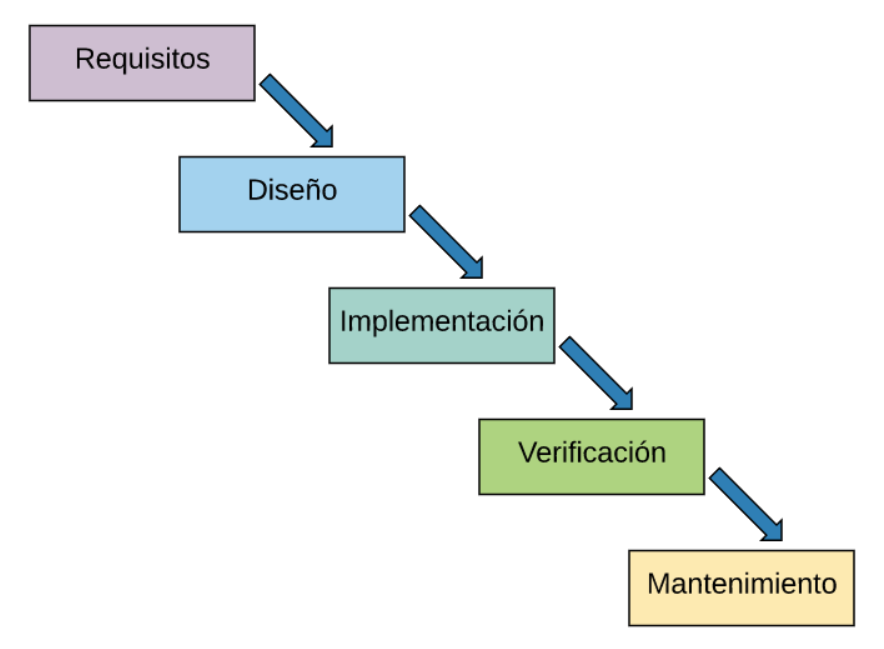
\includegraphics[width=5.00in]{images/desarrollo_cascada.PNG}
\caption{Las etapas del modelo en cascada.
 Recuperado de: https://openclassrooms.com/en/courses/4309151-gestiona-tu-proyecto-de-desarrollo/4538221-en-que-consiste-el-modelo-en-cascada}
\label{fig:tecnologias_populares}
\end{figure}

\lsection{Estructura del documento}

A lo largo del siguiente documento se irán explicando todas las fases del ciclo de vida de nuestro proyecto, además de tener una fase previa de análisis de estado del 
arte y una fase posterior de trabajos futuros y conclusiones:
\begin{itemize}
\item\textbf{Estado del arte - \autoref{chap:estadodelarte}}: breve introducción y análisis de la domótica en la actualidad.
\item\textbf{Análisis y diseño - \autoref{chap:analisisydisenosistema}}: a lo largo del capítulo tres se analizan los requisitos de nuestra aplicación y se diseña la arquitectura del sistema.
\item\textbf{Desarrollo del sistema - \autoref{chap:desarrollosistema}}: en este capítulo se describirán las tecnologías utilizadas para el desarrollo del sistema, y se detallarán 
algunos aspectos técnicos acerca de la implementación.
\item\textbf{Pruebas - \autoref{chap:pruebas}}: en este capítulo se detallarán las pruebas realizadas para comprobar el correcto funcionamiento
de nuestro sistema y la detección de posibles bugs.
\item\textbf{Trabajos futuros - \autoref{chap:trabajofuturo}}: análisis de posibles trabajos futuros para nuestro HUB.
\item\textbf{Conclusiones - \autoref{chap:conclusiones}}: conclusiones obtenidas a lo largo del trabajo.
\end{itemize}


\newpage \thispagestyle{empty} % Página vacía 

\chapter{Estado del arte}
\label{chap:estadodelarte}

\lsection{Introducción}

\lsection{Historia, nacimiento y evolucin.} \label{sec:historia}

\lsection{La anatoma del ojo}
\label{sec:anatomiaojo}
\subsection{Aspectos diferenciadores del iris}


\lsection{Adquisicin del Iris} \label{sec:adquisicion}
\subsection{Introduccin}
\subsection{Esquemas de adquisicin tradicionales}
\subsection{Consideraciones sobre la iluminacin}
\label{subsec:iluminacion}
\subsection{Posicionamiento del Iris}
\subsection{Sistemas comerciales de adquisicin}


\lsection{Localizacin y segmentacin del Iris} \label{sec:localizacion}
\subsection{Introduccin}
\subsection{Metodologa de J. Daugman y derivadas}
\subsection{Metodologa de R. Wildes y derivadas}
\subsection{Otras metodologas}
\subsection{Comparativa de metodologas}
\subsection{Deteccin de pestaas y ruido}


\lsection{Normalizacin del tamao}
\label{sec:normalizacion}
\subsection{Daugman's Rubber Sheet Model}
\subsection{Image Registration}
\subsection{Normalizacin en ngulo}
\subsection{Mejora del contraste y eliminacin de ruido}


\lsection{Algoritmos de Codificacin}
\label{sec:codificacion}
\subsection{Metodologa de Daugman: Filtros de Gabor}
\subsection{Metodologas alternativas a la de Daugman}
\subsubsection{Filtros Log-Gabor} \label{subsubsec:filtrosLogGabor}
\subsubsection{Wavelets}
\subsubsection{Haar Wavelet}
\subsubsection{Transformada Discreta del Coseno (DCT)}
\subsection{Metodologas de Wildes. Vectores de caractersticas reales (no binarios)}


\lsection{Algoritmos de Matching}
\label{sec:matching}
\subsection{Introduccin}
\subsection{Distancia de Hamming} 
\label{subsec:distHamming}
\subsection{Distancia eucldea ponderada}
\subsection{Correlacin normalizada}


\lsection{Problemtica y retos futuros}
\label{sec:problematica}
\subsection{Segmentacin}
\subsection{Captura ideal no invasiva}


\lsection{Competiciones o Evaluaciones de Iris}
\label{sec:competiciones}
\subsection{The Iris Challenge Evaluation (ICE)}
\subsection{The Noisy Iris Challenge Evaluation (NICE)}


\lsection{Bases de datos} \label{sec:databases}
\subsection{CASIA} \label{sec:CASIA_database}
\subsection{BioSec Baseline y BioSecurID} \label{sec:ATVS_database}



\newpage \thispagestyle{empty} % Pgina vaca 

\chapter{Diseño del sistema}
\label{chap:disenosistema}
En este capítulo se describirá el diseño del sistema desarrollado. 
En la sección 3.1 se detallará la arquitectura del sistema global. 
En el apartado 3.2 se profundizará en la arquitectura interna del HUB.
\lsection{Necesidades del sistema}
En esta sección se analizarán las necesidades de nuestro sistema y los dispositivos con los que nos comunicaremos.
\subsection{Necesidades de los dispositivos}
Antes de empezar a diseñar el sistema y elegir el protocolo que se utilizará y el medio físico por el que se comunicarán 
nuestros dispositivos es necesario analizar los dispositivos que podrán conectarse a nuestro HUB así como sus necesidades. 
Una vez determinados los requisitos del protocolo se estudiará el medio físico de comunicación.
\par
Los principales dispositivos domóticos que hemos encontrado son: sensores de temperatura, sensores de humedad, 
sensores de luz, sensores de movimiento, medidores de distancia, sensores de humo, sensores magnéticos, cámaras, 
bombillas, enchufes, termostatos, motores, aires acondicionados, interruptores y altavoces. Estos dispositivos
 pueden ser divididos en dos grupos: sensores y actuadores. 
\par
Los sensores solamente envían determinada información a nuestro HUB (comunicación unidireccional), 
mientras que los actuadores reciben mensajes con determinados comandos a parte de enviar información del estado 
en el que se encuentran (comunicación bidireccional).

Agrupación de los dispositivos encontrados:

\begin{figure}[H]
\centering
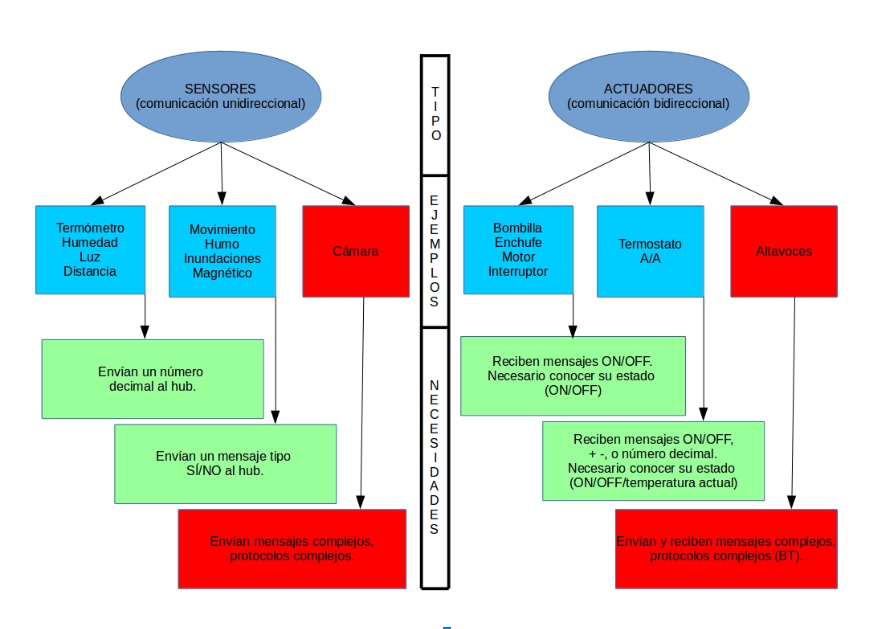
\includegraphics[width=6.00in]{images/descripcion_dispositivos.png}
\caption{Tipos de dispositivos}
\label{fig:descripcion_dispositivos}
\end{figure}


Para la definición del protocolo dividiremos los dispositivos en tres tipos:
\begin{itemize}
\item Tipo 1 (sensores): el hub sólo recibe información de los sensores. El hub no necesita saber qué tipo de información recoge (número decimal, SÍ/NO...etc), simplemente la actualiza y la muestra al usuario.
\item Tipo 2 (actuadores): estos dispositivos envían información al HUB y son capaces de recibir comandos tipo ON/OFF, +/-, número decimal...etc.
\item Tipo 3: cámaras IP. Este sensor recibirá un tratamiento especial debido a la necesidad de una comunicación constante y rápida.
\end{itemize}
\subsection{Necesidades del sistema}
Una vez analizadas las necesidades de los dispositivos podemos analizar las necesidades de nuestro sistema.
Para el desarrollo de nuestro sistema necesitaremos una arquitectura que nos permita:
\begin{itemize}
\item Comunicación bidireccional entre los dispositivos y el hub: es necesario que el hub conozca información de los dispositivos, 
registre dispositivos y gestione dispositivos, así como también es necesario que los dispositivos puedan recibir comandos provenientes
del hub. El hub debe permitir aceptar dispositivos con diferentes comandos, y no ceñirse sólo a un número cerrado de comandos (ON/OFF, +/-,...).
\item Comunicación entre el hub y la interfaz: será necesario que la información de los dispositivos y el estado de los mismos sea accesible
a través de la interfaz de usuario. Además el usuario debe ser capaz de gestionar los dispositivos y enviar comandos a los actuadores
a través de la interfaz.
\item Seguridad en la comunicación: es imprescindible que toda comunicación se realice de manera segura, de tal manera que nadie pueda modificar o
acceder a nuestra información.
\item Escalabilidad: aunque durante la realización de nuestro proyecto nos centraremos únicamente en la comunicación mediante protocolo HTTPS, 
es necesario diseñar un sistema escalable que el día de mañana pueda funcionar con diferentes protocolos y dispositivos.
\end{itemize}
\lsection{Protocolos}
En esta sección se describirá el protocolo que se utilizará en las comunicaciones entre los dispositivos y el HUB.
\subsection{Protocolo HTTPS}
El protocolo elegido para la comunicación entre dispositivos, hub e interfaz es el protocolo HTTPS (Hypertext Transfer Protocol Secure).
\par
Este protocolo nos da la posibilidad de implementar una API REST consumible por parte de los dispositivos y por parte de la interfaz,
sin necesidad de utilizar diferentes protocolos para los diferentes canales.
\par
Las APIs REST están muy estandarizadas a día de hoy y nos dan la capacidad de separar lógica y funcionalidad entre cliente y servidor y de ser capaces
de utilizar diferentes lenguajes y tecnologías para cada lado. Es decir, podemos tener un servidor escrito en Express.js (JavaScript), una interfaz 
gráfica utilizando Angular5 (TypeScript), y unos actuadores/sensores que utilicen CherryPy (Python).
\par
Además, utilizar HTTPS nos ofrece la posibilidad de crear un canal de comunicación cifrado, de manera que la información que circula en dicho 
canal no pueda ser descifrada por ningún intermediario ni se pueda sufrir un ataque Man-In-The-Middle*.
\lsection{Arquitectura del sistema}
En esta sección se describirá el diseño y la arquitectura del sistema de manera global, incluyendo dispositivos actuadores, 
dispositivos sensores y el propio hub.
\subsection{Arquitectura del sistema}
Teniendo en cuenta las necesidades de nuestro sistema realizaremos una arquitectura similar a las arquitecturas de microservicios,
en la que el hub y los actuadores serán los hosts de un servidor REST y serán capaces de recibir y procesar peticiones.
\par
El hub recibirá peticiones de parte de la interfaz de usuario y de los dispositivos, y lanzará peticiones a los actuadores.
Para ello se establecerán dos APIS publicadas por el HUB y consumibles por la interfaz de usuario y los dispositivos:
\begin{itemize}
\item \underline{Interface API:} será consumida por la interfaz de usuario. Se encargará de enviar la información de los dispositivos al usuario: número
 de dispositivos, localización, etc... Además, permitirá al usuario gestionar dispositivos y enviarles comandos.
\item \underline{Sensors API:} será consumida por actuadores y sensores por igual. Permitirá a los dispositivos darse de alta en el sistema y actualizar
periódicamente su información.
\end{itemize}
Los actuadores, además de lanzar peticiones al hub para informar de su estado, deberán ser capaces de recibir peticiones del hub con
diferentes comandos. Para ello se establecerá otra API que todos los dispositivos deberán seguir, para que así el HUB consuma la misma API
en los diferentes dispositivos. Será denominada en adelante como \underline{Actuators API}. Estableceremos y explicaremos estas APIs en los capítulos siguientes.
\par
Todas las peticiones deben ser securizadas, y debemos asegurar que ningún intruso pueda acceder y/o modificar la información de nuestro sistema.

Esquema de la arquitecura a seguir:
\begin{figure}[H]
\centering
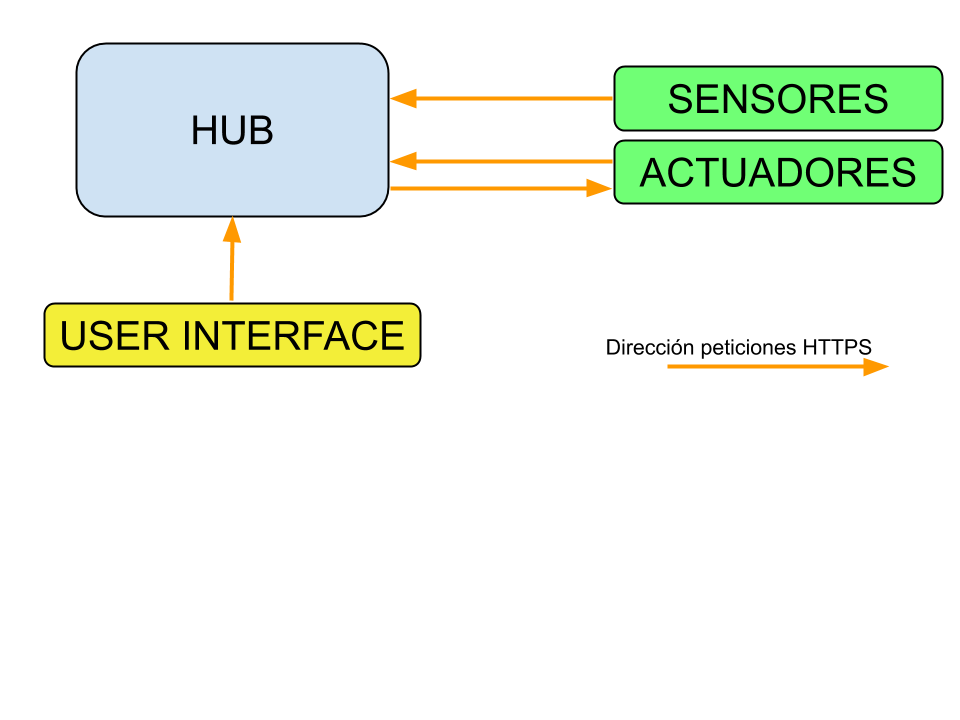
\includegraphics[width=6.00in]{images/esquema_arquitectura.png}
\caption{Tipos de dispositivos}
\label{fig:descripcion_dispositivos}
\end{figure}

\subsection{Modelo de datos}
En esta sección se describirán los modelos de datos a utilizar. Todos los datos residirán en el HUB, que será el encargado de orquestarlos,
organizarlos y mantenerlos.
\par
Analizando las necesidades del sistema nos encontramos con cuatro entidades a definir:
\begin{itemize}
\item \underline{Dispositivos}: esta entidad se utilizará para almacenar la información de los actuadores/sensores. En el caso de los actuadores,
será necesario guardar su dirección IP, para poder enviarles comandos.
\item \underline{Comandos}: entidad para almacenar los comandos de los diferentes dispositivos. Cada comando tendrá un código y una descripción.
\item \underline{Habitaciones}: esta entidad nace de la necesidad de organizar los dispositivos de una casa en grupos más pequeños. Una manera lógica 
y muy común es por habitaciones, cada dispositivo podrá o no pertenecer a una habitación.
\item \underline{Usuarios}: es necesario restringir los usuarios que pueden tener acceso a nuestro sistema. Para ello existirán distintos usuarios, pudiendo
dar de alta nuevos usuarios y modificar los existentes. Todos los usuarios tendrán permisos en el sistema, sin existir roles de usuario. 
\par
Diagrama entidad-relación modelo de datos:
\begin{figure}[H]
\centering
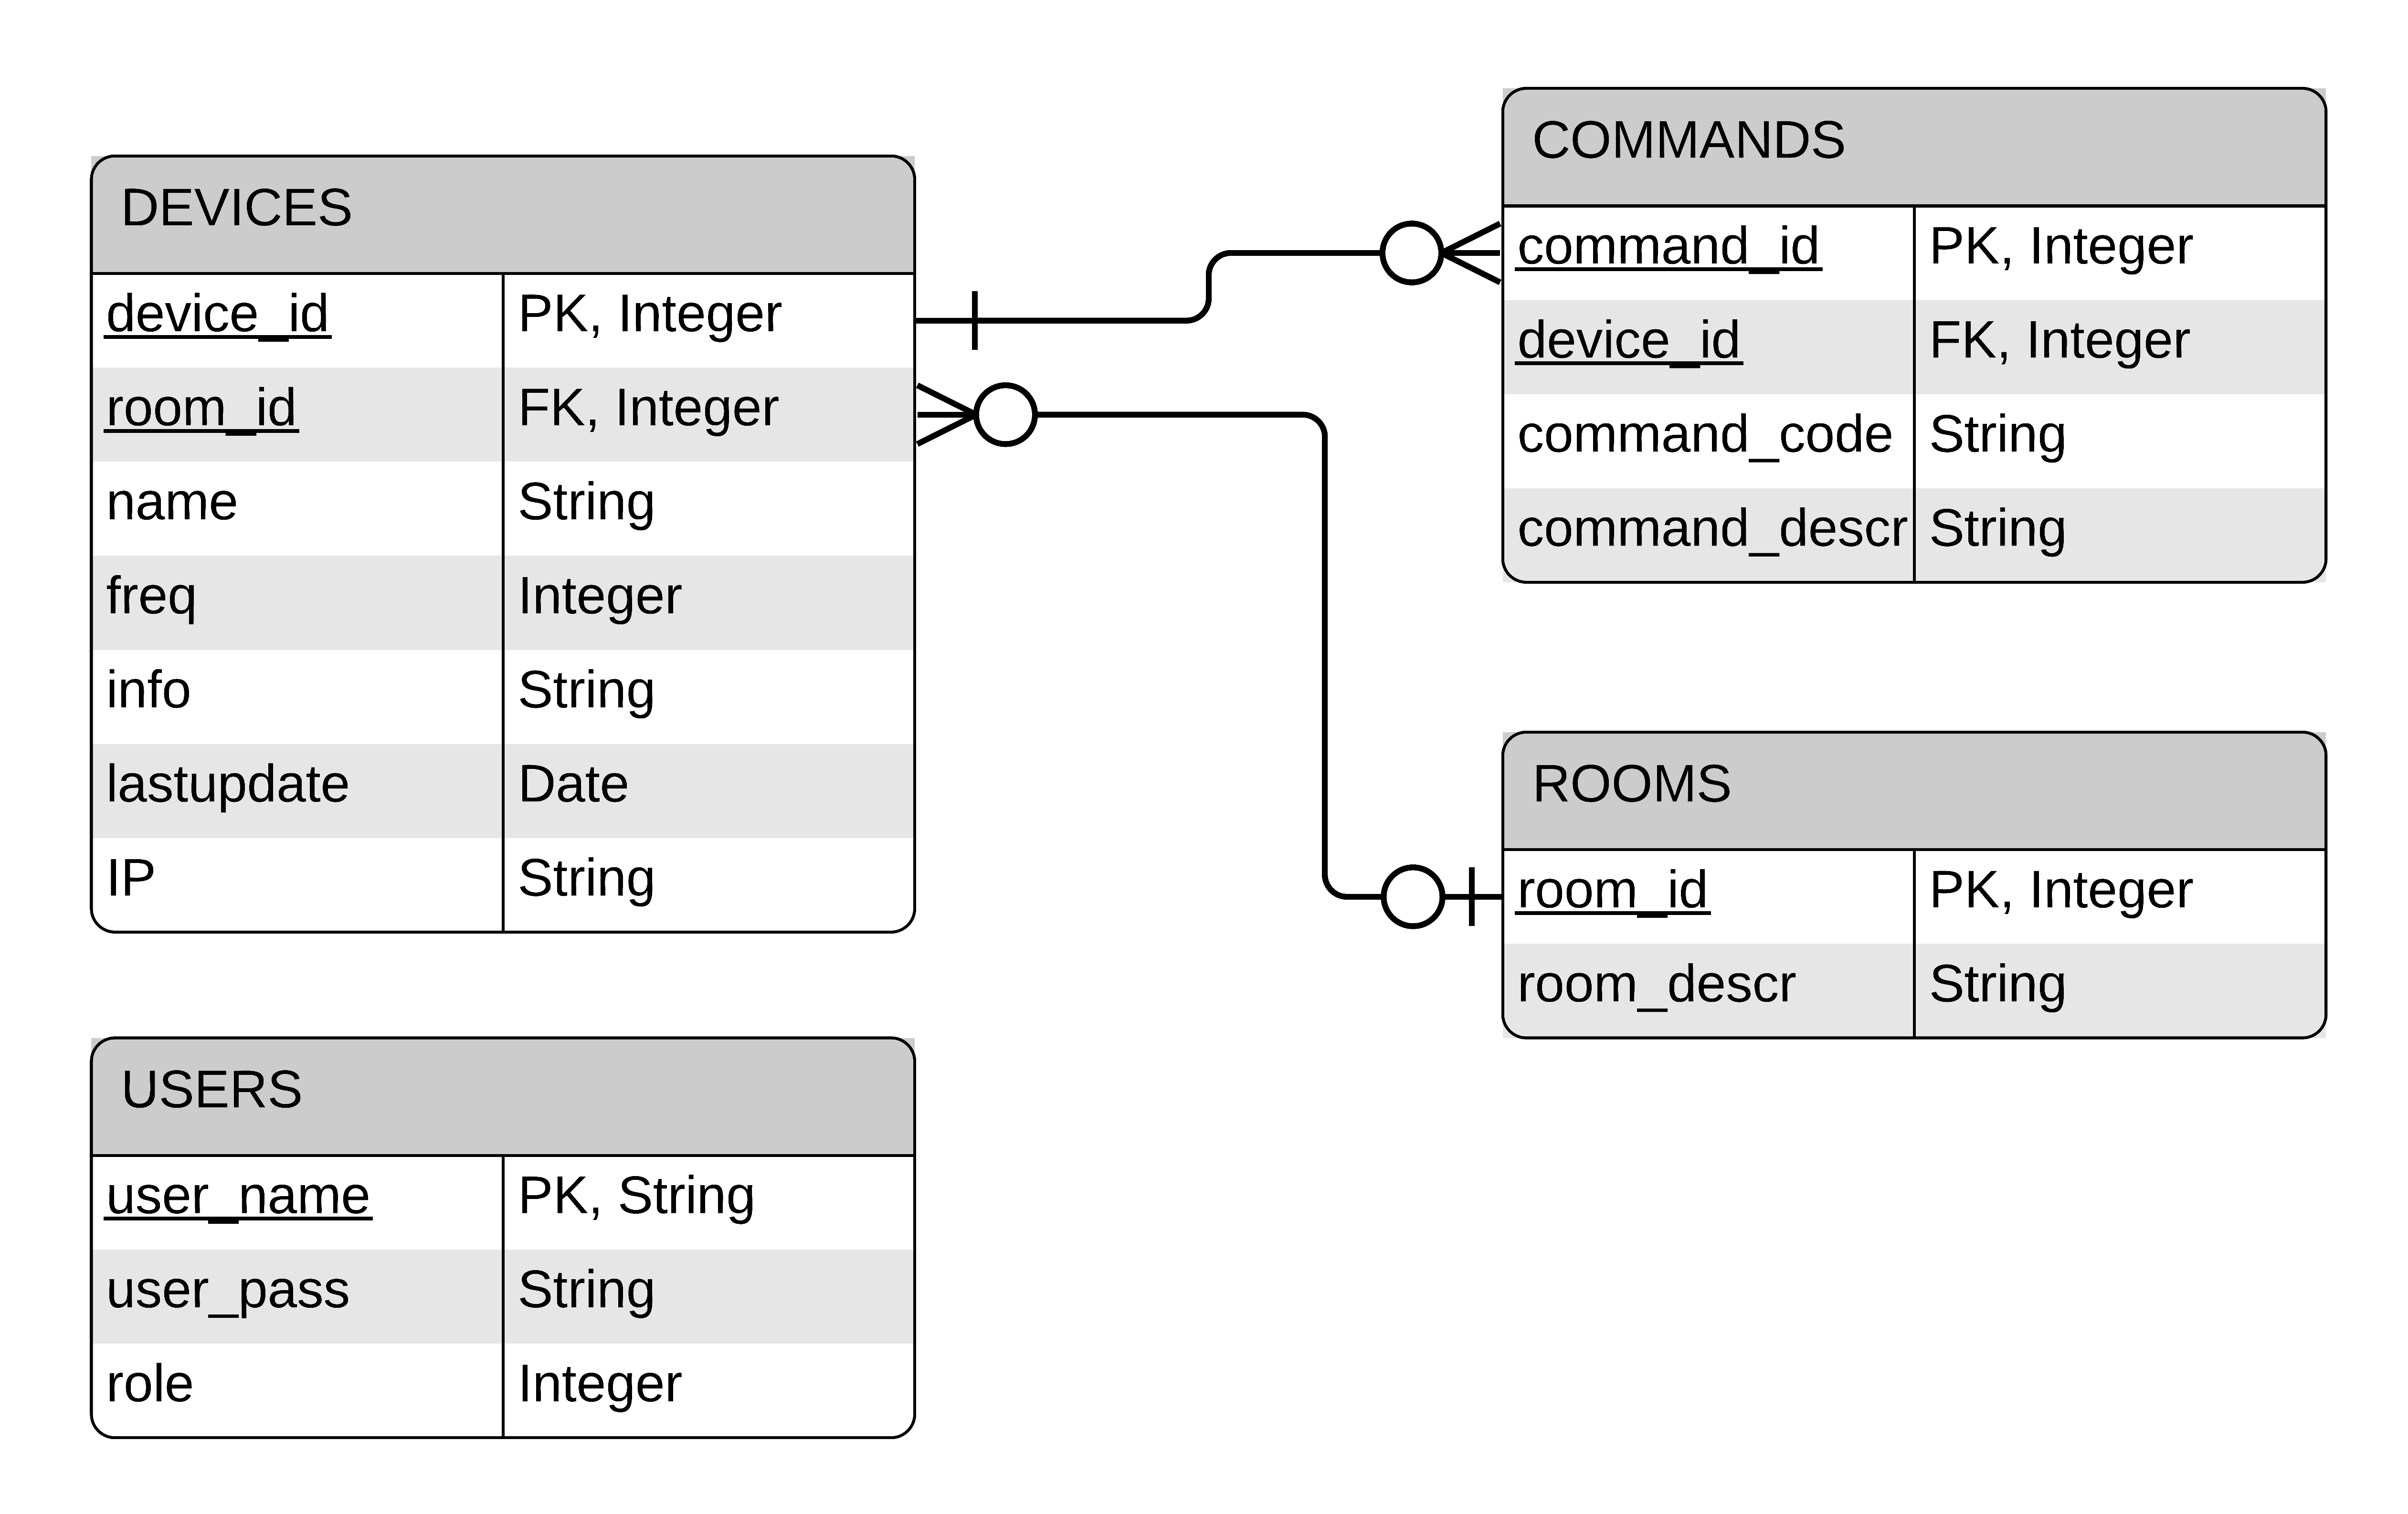
\includegraphics[width=6.00in]{images/er_brimo.png}
\caption{Diagrama ER}
\label{fig:diagrama-er}
\end{figure}

\end{itemize}
\subsection{APIS}
Una vez numeradas las diferentes APIS a utilizar y definido el modelo de datos podemos comenzar a definir detalladamente cada una de las APIS.
Al tratarse de APIS REST, en la definición
de cada método es necesario informar: ruta del método, verbo (GET, POST, PUT, PATCH, DELETE), cuerpo de la petición (si existiera) y variables
de la ruta (si existieran).
\par
A no ser que se indique lo contrario, el cuerpo de todas las peticiones debe estar en formato JSON, y debe ser
informada la cabecera \textbf{Content-Type} con valor \textbf{application/json}.
\par
Como se ha descrito anteriormente todas las peticiones deberán ir securizadas, para lo que se utilizarán tokens JWT. Es imprescindible que el
token vaya en la cabecera \textbf{x-access-token} de cada petición, o de lo contrario la petición será denegada. La generación de tokens y la gestión
de usuarios es descrita por la API de login.
\par
Estas APIS funcionan como contratos entre publicador y consumidor, y es imprescindible que ambas partes consuman y publiquen de la 
manera acordada para que el sistema completo funcione. El cambio de uno de estos contratos debe ser indicado a todas las partes para que se tenga
en cuenta en los desarrollos futuros.
\par
Todos los métodos de estas APIs están enumerados y definidos en un proyecto de Postman desde el cual se pueden probar.
\par
\subsubsection{Sensors API}
Esta API será consumida tanto por sensores como por actuadores, y les permitirá registrarse en el sistema y actualizar su información.

\begin{itemize}
\item \textbf{POST /brimo/sensors-api/devices}: se utilizará para el registro de dispositivos. En el cuerpo de la petición se informarán
 un nombre descriptivo (podrá ser modificado por el usuario más adelante) y frecuencia
de actualización de la información \footnote{ Si el dispositivo pasa más de los segundos informados sin actualizar información, entonces
el HUB lo considerará desconectado.}. Opcionalmente, en el caso de ser un actuador, el dispositivo informará de los comandos que es capaz
de recibir. Estos comandos vendrán en forma de array y deben contener descripción y código de comando.
Si el registro es correcto el HUB responderá con un 201 CREATED y un id de dispositivo. Este id será utilizado por el dispositivo más adelante
para enviar información al HUB.
\item \textbf{PUT /brimo/sensors-api/devices/\{device-id\}/info}: se utilizará para actualizar la información del dispositivo. El parámetro
device-id indicará el id del dispositivo, proveniente del registro. Si la información se actualiza correctamente el HUB devolverá 200 OK. Una vez
actualizada la información del dispositivo se actualizará la hora de última actualización \textbf{(lastupdate)}.
\end{itemize}

\subsubsection{Actuators API}
Esta API será consumida por el HUB, y permitirá al HUB enviar comandos a los dispositivos.

\begin{itemize}

\item \textbf{POST /brimo/actuators-api/commands?command\_code=ON}: es el único método de la API. El HUB enviará esta petición para enviar
comandos al dispositivo. El código de comando debe haber sido informado previamente en la fase de registro.

\end{itemize}

\subsubsection{Interface API}
Como hemos explicado anteriormente, esta API será consumida por la interfaz de usuario y permitirá al usuario obtener información de los dispositivos,
gestionarlos y mandarles comandos:

\begin{itemize}
\item \textbf{GET /brimo/interface-api/devices}: esta petición nos devolverá información de todos los dispositivos
dados de alta en el sistema. Al tratarse de una lista no se poblarán todos los campos del dispositivo, sólo los comunes: id del dispositivo, nombre,
frecuencia, fecha de última actualización de la información, id de habitación y descripción de la habitación.
\item \textbf{GET /brimo/interface-api/devices/\{device-id\}}: a diferencia de la petición anterior, se obtiene únicamente la información
del dispositivo indicado con el parámetro device-id. Esta información es más completa, y además de la información de la petición anterior
se obtiene la lista de comandos que acepta el dispositivo y su IP.
\item \textbf{DELETE /brimo/interface-api/devices/\{device-id\}}: a través de esta petición el usuario podrá eliminar el dispositivo indicado. A partir
de este momento el sistema denegará al dispositivo la comunicación con el mismo.
\item \textbf{PATCH /brimo/interface-api/devices/\{device-id\}/?room-id=12\&name=sensor-habitacion}: esta petición permitirá editar la habitación
en la que se encuentra el dispositivo y su nombre. Ambos parámetros room-id y name son opcionales, aunque al menos uno debe estar presente.
\item \textbf{DELETE /brimo/interface-api/devices/\{device-id\}}: a través de esta petición el usuario podrá eliminar el dispositivo indicado. A partir
de este momento el sistema denegará al dispositivo la comunicación con el mismo.
\item \textbf{PATCH /brimo/interface-api/devices/\{device-id\}/?room-id=12\&name=sensor-habitacion}: esta petición permitirá editar la habitación
en la que se encuentra el dispositivo y su nombre. Ambos parámetros room-id y name son opcionales, aunque al menos uno debe estar presente.
\item \textbf{POST /brimo/interface-api/devices/\{device-id\}/commands?command-code=ON}: se utilizará para enviar comandos al dispositivo informado.
La petición irá al HUB, que será el encargado de enviar otra solicitud al dispositivo correspondiente. Para ello, utilizará la IP del dispositivo.
\item \textbf{GET /brimo/interface-api/devices/rooms}: devolverá la lista actual de habtiaciones registradas. Se devolverán en forma de 
array y en cada una de ellas vendrán informadas descripción e identificador.
\item \textbf{POST /brimo/interface-api/devices/rooms}: se utilizará por el usuario para añadir habitaciones. Únicamente es necesario informar
el nombre de la nueva habitación. Si el registro de la habitación es correcto, entonces el HUB devolverá 201 CREATED con el id de la nueva habitación.

\end{itemize}


\subsubsection{Login API}
Esta API será utilizada para la generación de los JWT, que necesariamente, deben ir informados en las cabeceras de cada petición. Además, gestionará
los usuarios con acceso al sistema.
\begin{itemize}
\item \textbf{POST /brimo/login-api}: se deberán informar los campos usuario y contraseña para la correcta generación del token. En el caso
de introducir credenciales inválidas el HUB devolverá 401 Unauthorized. En caso de éxito el HUB devolverá el token generado, que será válido
para las siguientes dos horas.
\item \textbf{POST /brimo/login-api/users}: servirá para añadir nuevos usuarios al sistema. Deberán informarse nombre de usuario y contraseña.
\item \textbf{PUT /brimo/login-api/users}: servirá para modificar la contraseña y/o el nombre de usuario actuales. Deberán ir informados en el
cuerpo de la petición al menos uno de los dos parámetros.
\end{itemize}

\lsection{Arquitectura del hub}
En esta sección definiremos los módulos que nuestro HUB deberá tener y las funciones que cada uno debe cumplir. La organización por módulos, además
de permitirnos organizar nuestro software de una manera clara, nos ayudará a añadir nuevos módulos y funcionalidad el día de mañana.
\par
Por ejemplo, en el módulo de servicios residirá toda la lógica interna, mientras que el enrutadors será el módulo encargado de "traducir" los datos
provenientes de la red a un modelo de datos conocido e invocar a los diferentes servicios. De esta forma, si en un trabajo futuro queremos añadir
dispositivos bluetooth crearemos un módulo bluetooth que reutilice nuestros servicios.
\par
Otro ejemplo sería la migración de nuestra base de datos a otro motor diferente; sólo necesitaríamos cambiar el módulo repositorio, el resto del sistema
se mantendría intacto.
\par
Cada módulo
debe ser independiente del resto, y la modificación interna de un módulo no debería requerir la modificación del resto de módulos.
\subsection{Módulo enrutador}
Este módulo será el encargado de gestionar las conexiones entrantes y de manejar la información proveniente del exterior. Para nuestro caso, que utilizaremos
el protocolo HTTPS, en este módulo residirán las implementaciones de las APIS anteriormente definidas. Se encargará de implementar todas las rutas, encapsular
los diferentes parámetros en objetos de nuestro modelo y enviar las respuestas y códigos necesarios tras la invocación al módulo de servicios.
\subsection{Módulo middleware}
A pesar de haber separado este módulo del módulo enrutador, este módulo está totalmente ligado a la utilización del protocolo HTTPS. 
Se trata de un módulo totalmente independiente del módulo enrutador, y tendrá dos funciones principales: 
interceptar las peticiones antes de que lleguen al
\begin{itemize}
\item Interceptar todas las peticiones antes de que lleguen al enrutador y validar las cabeceras y el token JWT. Si el token no es válido entonces
se envía un 401 Unauthorized sin llegar al enrutador.
\item Interceptar los errores que se provoquen durante la ejecución del programa (independientemente del módulo) y traducirlos a respuestas HTTPS. Para esto 
será necesario utilizar un modelo común de error, que pueda ser interceptado por este módulo.
\end{itemize}
\subsection{Módulo de servicios}
En este módulo residirá la totalidad de nuestra lógica de negocio. A este módulo ya llegan objetos modelados con nuestro modelo de datos, y es totalmente
independiente del protocolo utilizado. Se encargará de hacer llamadas a los repositorios correspondientes y de aplicar la lógica correspondiente.
\par
Un ejemplo de lógica sería el registro de dispositivos; una vez recibido un dispositivo y sus correspondientes comandos y el servicio se encargará de hacer
las comprobaciones correspondientes y guardar primeramente el dispositivo y más adelante los comandos.
\par
Además, el módulo de servicios transformará los posibles errores provenientes de los repositorios para encapsularlos en errores internos. Un ejemplo sería
transformar un error 14 SQLITE\_CANT\_OPEN en el siguiente error: ``Error 01: no se ha podido acceder a la base de datos sqlite``.
\par
Tanto la entrada como la salida de datos de los métodos de nuestros servicios seguirán el modelo de datos del HUB.
\subsection{Módulo repositorio}
Este módulo contendrá toda la gestión de los datos del HUB. Será invocado por el módulo de servicios, y 
será el encargado de gestionar las conexiones con la base de datos e insertar/obtener datos de la misma.
Este módulo recibe datos modelados con nuestro modelo de datos, pero no necesariamente la manera de enviarlos/guardarlos tiene que coincidir con nuestro modelo 
de datos. Sin embargo, el retorno de los métodos de este módulo si serán datos modelados.
\par
Si en un futuro se realizasen llamadas a terceros, una API de Google por ejemplo, las llamadas a esa API se realizarían desde este módulo.
\subsection{Vista general}
Por lo tanto, el diseño esquemático de la arquitectura interna del hub sería el siguiente:
\begin{figure}[H]
\centering
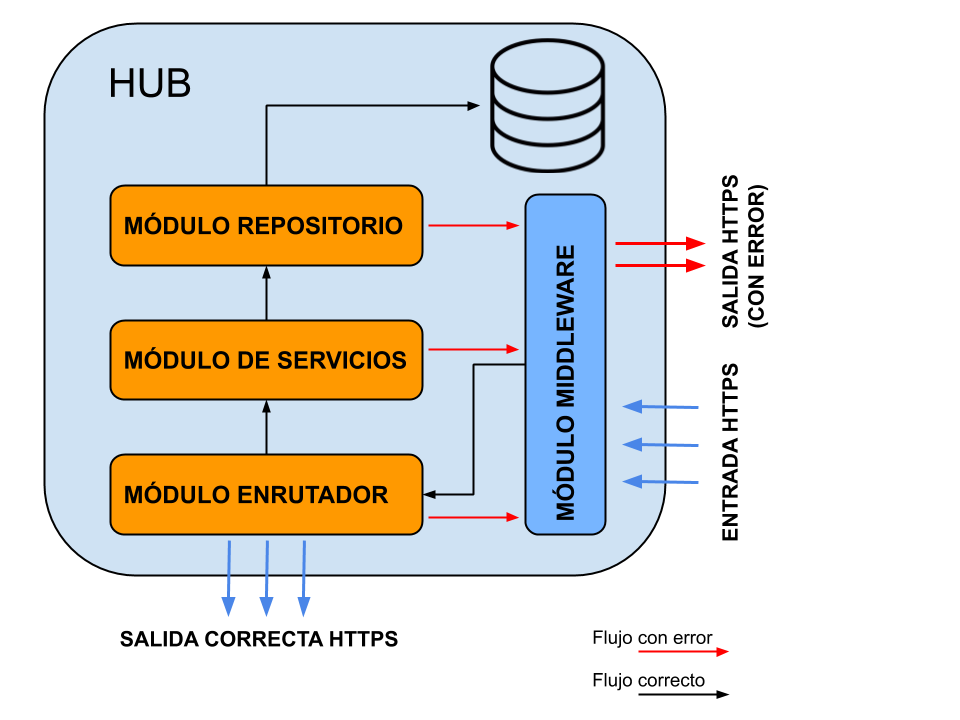
\includegraphics[width=6.00in]{images/arquitectura_hub.png}
\caption{Arquitectura interna del hub}
\label{fig:arquitectura_hub}
\end{figure}


\chapter{Desarrollo del sistema}
En este capítulo se explicarán las tecnologías utilizadas y las arquitecturas internas de cada subsistema. Los dos subsistemas que desarrollaremos
serán el HUB y la Interfaz gráfica.
\label{chap:desarrollosistema}
\lsection{Stack tecnológico}
Elegir el stack tecnológico a utilizar en el desarrollo de cualquier sistema es siempre una tarea difícil y determinante en el desarrollo de 
cualquier proyecto. Una elección inacertada puede significar el fracaso de un proyecto, mientras que una elección acertada sginificará que el 
proyecto salga adelante cumpliendo con todas las expectativas.
\par
Para elegir el stack correcto necesitamos tener en cuenta varios aspectos:
\begin{itemize}
\item\underline{Madurez de la tecnología:} es importante utilizar una tecnología con cierta madurez para evitar bugs, incompatibilidades, etc. Además, es
conveniente optar siempre por versiones LTS y evitar versiones Beta.
\item\underline{Comunidad/respaldo de la tecnología:} por lo general, este punto está muy relacionado con el punto anterior, ya que cuanta más madurez tiene
una tecnología, más comunidad suele existir. Aunque no sólo la madurez influye, también la popularidad de la tecnología, cuanto más se use esa tecnología,
más comunidad tiene. La comunidad de una tecnología, junto con su documentación, ayudan al desarrollador a enfrentarse a los problemas que surgen a lo
largo del desarrollo, siendo capaces de ver o preguntar a otros desarrolladores que ya se hayan enfrentado a dicho problema.
\item\underline{Conocimiento de los desarrolladores:} este punto es esencial, ya que es necesario que el equipo de desarrollo conozca las tecnologías, o en caso
contrario, ser capaces de contratar nuevos desarrolladores que sí las conozcan. La popularidad de la tecnología es esencial en este punto, ya que, por 
lo general, es más sencillo encontrar desarrolladores que conozcan tecnologías populares.
\item\underline{Librerías externas:} junto a la comunidad, las librerías externas ayudan a los desarrolladores a solucionar problemas que ya han sido resueltos
por otros desarrolladores. Por ejemplo, librerías para el manejo de fechas, librerías para gestionar conexiones con bases de datos...etc.
\item\underline{Licencias/mantenimiento de la tecnología:} es necesario tener en cuenta las licencias y el mantenimiento de las tecnologías antes de elegirlas,
pues pueden suponer gastos bastante elevados.
\end{itemize}

Teniendo en cuenta los apartados anteriores, se ha optado por utilizar Express.js junto sqlite para el desarrollo del HUB, e Ionic para el desarollo de
la interfaz gráfica.

\begin{figure}[H]
\centering

\includegraphics[width=5.00in]{images/stack_tecnologico.png}
\caption{Stack tecnológico escogido}
\label{fig:stack_teconologico}
\end{figure}

\subsection{Express.js}
Se trata de un framework open source para Node.js enfocado en el desarrollo de aplicaciones web. Utiliza JavaScript como lenguaje principal, un lenguaje moderno, muy popular y
muy rápido en ejecución. Los desarrolladores de Express.js definen a su framework como: \textit{``Infraestructura web rápida, minimalista, y flexible para Node.js``}.
Además, según \textbf{hackr.io}: \textit{``Express es uno de los frameworks que más rapido está creciendo en popularidad, y es utilizado por compañías como Accenture, IBM o
Uber``}.
\par
Al ser un framework para Node, podemos utilizar librerías de terceros de manera sencilla a través del gestor de paquetes NPM. La comunidad de Node es una de las comunidades más activas
y grandes que existen.
\newpage
Según el \textbf{Developer Survey 2018} realizado por \textbf{StackOverFlow}, una de las comunidades de desarrolladores más grandes del mundo, JavaScript es la tecnología
 más popular (con un 71.5\%) dentro de las tecnologías de programación, scripting y lenguajes marcados:

\begin{figure}[H]
\centering
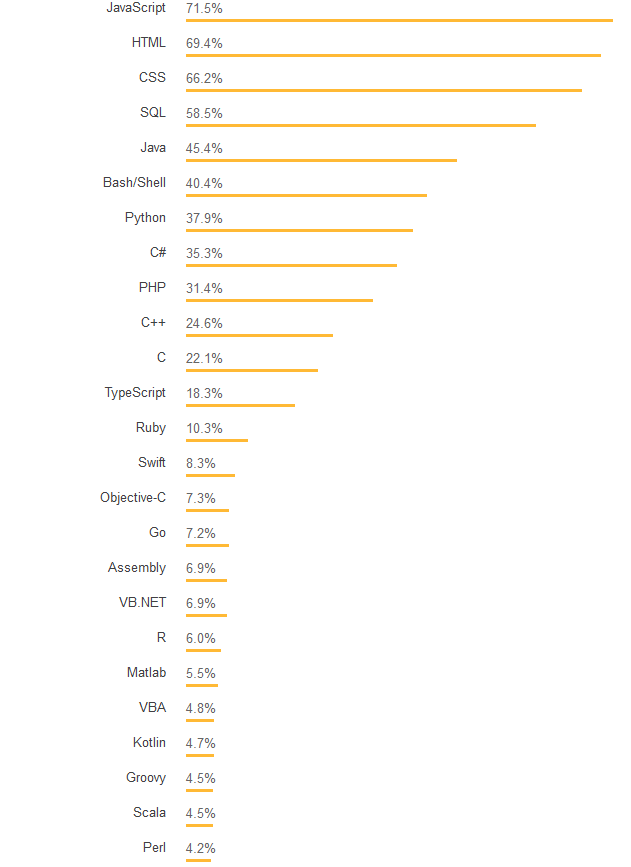
\includegraphics[width=5.00in]{images/tecnologias_populares.png}
\caption{Developer Surver Results 2018. Most popular programming, scripting and markup languagaes technologies.
 Recuperado de: https://insights.stackoverflow.com/survey/2018\#technology-\_-programming-scripting-and-markup-languages}
\label{fig:tecnologias_populares}
\end{figure}

\newpage
Además, el mismo estudio revela que Node.js es la tecnología más popular (con un 49.9\%) dentro del apartado de frameworks, librerías y herramientas:

\begin{figure}[H]
\centering
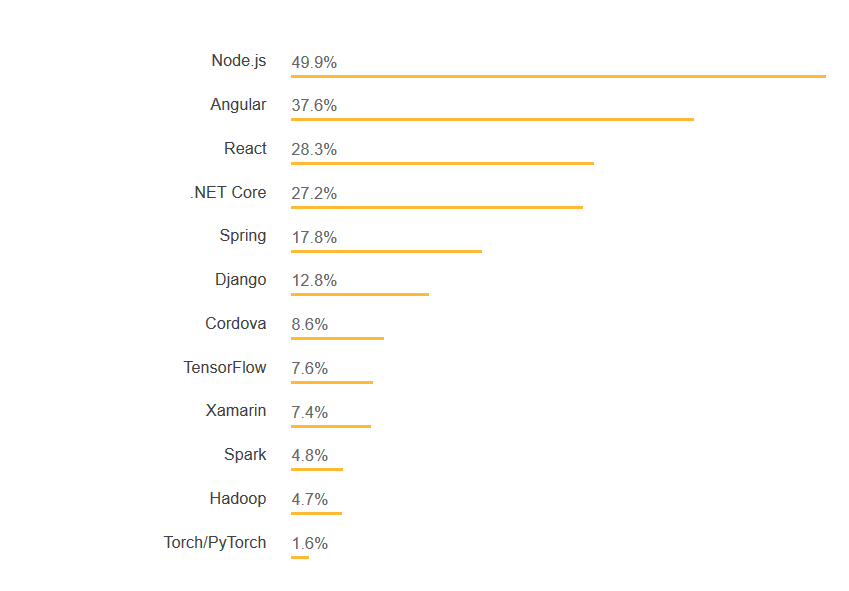
\includegraphics[width=6.00in]{images/frameworks_populares.png}
\caption{Developer Surver Results 2018. Most popular frameworks, libraries and tools. 
Recuperado de: https://insights.stackoverflow.com/survey/2018\#technology-\_-programming-scripting-and-markup-languages}
\label{fig:frameworks_populares}
\end{figure}

\subsection{SQLite}
SQLite es una librería open source que implementa un pequeño gestor de bases de datos SQL. No necesita ejecutarse en un servidor a parte, lee y escribe
directamente de un fichero. Es perfecto para nuestro caso, en el que no se necesitan muchas tablas y éstas no contendran demasiados datos. Todo esto hace
que SQLite se adapte muy bien para sistemas ligeros.
\par
La no necesidad de ejecución en paralelo significa que apenas requiere configuración. Por otro lado, es una librería muy compacta y bastante madura, con 
inicios en el año 2000. Basándonos de nuevo en el \textbf{Developer Survey 2018}, SQLite es el quinto gestor de bases de datos preferido por los desarrolladores,
con un 19.7\%, por delante de gestores muy conocidos como Redis, ElasticSearch, MariaDB u Oracle.
\par
La madurez y popularidad de este gestor hace, como era de esperar, que tenga total compatibilidad con Node.js, y por lo tanto con Express, gracias al módulo
NPM \textbf{sqlite3}.

\subsection{Ionic}
Ionic es un framework open source que nos permite construir aplicaciones híbridas de manera rápida y sencilla. Una aplicación híbrida es, realmente, una
aplicación web que se ejecuta en un WebView dentro del dispositivo, aunque pueden tener acceso directamente a las APIs nativas del dispositivo: GPS, almacenamiento, 
contactos...etc.
\par
La principal ventaja de Ionic es que el mismo desarrollo genera aplicaciones Android, IOS y Web, ya que se trata de aplicaciones web embebidas en un WebView. Además,
Las aplicaciones Ionic están hechas por componentes reutilizables, e Ionic nos ofrece muchísimos componentes (``UI Components``) para construir la interfaz de nuestra
aplicación de manera rápida: botones, alertas, menús, indicadores de carga...etc.
\par
Ionic utiliza tecnologías Web para el desarrollo: TypeScript, HTML y CSS, lo que facilita mucho la migración de una aplicación móvil a una versión web y viceversa: la
mayoría de servicios y lógica puede ser reutilizada, cambiando únicamente los componentes que se utilizan.
\par
Al no tratarse de aplicaciones nativas, Ionic no es indicado para aplicaciones complejas, ya que el rendimiento y la gestión de recursos es mucho menos óptima en
este tipo de aplicaciones. Sin embargo, no es nuestro caso, ya que necesitamos una aplicación sencilla, con una interfaz sencilla que pueda hacer peticiones fácilmente
a una API REST, por lo que Ionic encaja a la perfección.
\par
Además, Ionic ofrece ``live reloading``: no es necesario recompilar o volver a ejecutar nuestra aplicación, si no que los cambios son detectados en caliente y se actualiza
automáticamente.
\lsection{Hub}
Como ya se ha explicado anteriormente, el HUB es la parte central de nuestro sistema. En él reside toda la lógica de negocio, y es el encargado
de comunicarse con la interfaz y los dispositivos.
\subsection{Módulos}
En esta sección se definirán los módulos del HUB y las funciones que cumplen cada uno de ellos. La organización por módulos, además
de permitirnos organizar nuestro software de una manera clara, nos ayuda a construir software flexible: en futuras mejoras del HUB se podrán añadir
nuevos módulos y funcionalidades con facilidad.
\par
Por ejemplo, en el módulo de servicios reside toda la lógica interna, mientras que el módulo enrutador es el encargado de ``traducir`` los datos
provenientes de la red a un modelo de datos conocido e invocar a los diferentes servicios. De esta forma, si en un trabajo futuro queremos añadir
dispositivos bluetooth crearemos un módulo bluetooth que reutilice nuestros servicios.
\par
Otro ejemplo sería la migración de nuestra base de datos a otro motor diferente; sólo necesitaríamos cambiar el módulo repositorio, el resto del sistema
se mantendría intacto.
\par
Cada módulo debe ser independiente del resto, y la modificación interna de un módulo no debería requerir la modificación del resto de módulos.
\subsection{Módulo enrutador}
Este módulo es el encargado de gestionar las conexiones entrantes y de manejar la información proveniente del exterior. Para nuestro caso, que utilizamos
el protocolo HTTPS, en este módulo residirán las implementaciones de las APIS anteriormente definidas. Se encarga de implementar todas las rutas, encapsular
los diferentes parámetros en objetos de nuestro modelo y enviar las respuestas y códigos necesarios tras la invocación al módulo de servicios.
\subsection{Módulo middleware}
A pesar de haber separado este módulo del módulo enrutador, este módulo está totalmente ligado a la utilización del protocolo HTTPS. 
Se trata de un módulo totalmente independiente del módulo enrutador, y tiene dos funciones principales:
\begin{itemize}
\setlength\itemsep{6pt plus 1pt minus 1pt}
\item Interceptar todas las peticiones antes de que lleguen al enrutador y validar las cabeceras y el token JWT. Si el token no es válido entonces
se envía un 401 Unauthorized sin llegar al enrutador.
\item Interceptar los errores que se provoquen durante la ejecución del programa (independientemente del módulo) y traducirlos a respuestas HTTPS. Para esto 
es necesario utilizar un modelo común de error que pueda ser interceptado por este módulo.
\end{itemize}
\subsection{Módulo de servicios}
En este módulo reside la totalidad de nuestra lógica de negocio. A este módulo ya llegan objetos modelados con nuestro modelo de datos, y es totalmente
independiente del protocolo utilizado. Se encarga de hacer llamadas a los repositorios y de aplicar la lógica correspondiente en cada uno de los casos.
\par
Un ejemplo de esta lógica es el registro de dispositivos; una vez recibido un dispositivo y sus correspondientes comandos, el servicio se encarga de hacer
las comprobaciones correspondientes y guardar el dispositivo y después sus comandos.
\par
Además, el módulo de servicios transforma los posibles errores provenientes de los repositorios para encapsularlos en errores internos. Un ejemplo sería
transformar un error \textbf{``14 SQLITE\_CANT\_OPEN``} en el siguiente error: \textbf{``Error 01: no se ha podido acceder a la base de datos sqlite``}.
\par
Tanto la entrada como la salida de datos de los métodos de nuestros servicios seguirán el modelo de datos del HUB.
\subsection{Módulo repositorio}
Este módulo contiene toda la gestión de los datos del HUB. Es invocado por el módulo de servicios, y 
es el encargado de gestionar las conexiones con la base de datos e insertar/obtener datos de la misma.
Este módulo recibe datos modelados con nuestro modelo de datos, pero no necesariamente la manera de enviarlos/guardarlos tiene que coincidir con nuestro modelo 
de datos. Sin embargo, el retorno de los métodos de este módulo sí serán datos modelados.
\par
Si en un futuro se realizasen llamadas a terceros, una API de Google por ejemplo, las llamadas a esas APIS también se realizarían desde este módulo.
\subsection{Vista general}
Por lo tanto, el diseño esquemático de la arquitectura interna del hub es el siguiente:
\begin{figure}[H]
\centering
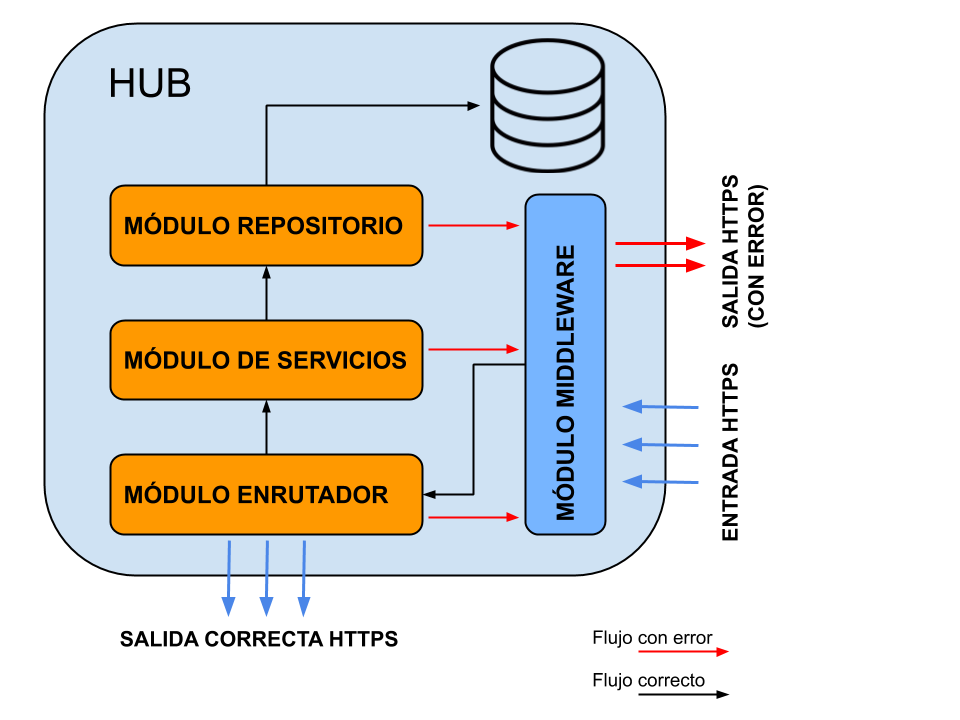
\includegraphics[width=6.00in]{images/arquitectura_hub.png}
\caption{Arquitectura interna del hub}
\label{fig:arquitectura_hub}
\end{figure}
\subsection{Seguridad}
\lsection{Interfaz}
En esta sección se describirán los distintos componentes y pantallas que nuestra aplicación tendrá así como los diferentes servicios. 
\subsection{Pantallas}
Como se ha explicado anteriormente, una de las grandes ventajas de Ionic es la enorme cantidad de UI Components ya hechos que nos ofrece.
En esta sección, se explicarán las pantallas de la aplicación y el flujo entre ellas, y se explicarán los componentes utilizados para cada
una de ellas.
\subsubsection{Diagrama de flujo de las pantallas}
Un diagrama de flujo nos ayuda a entender la navegabilidad de nuestra aplicación. Para evitar sobrecargar el diagrama se han omitido todas
las pantallas que consisten en ``pop-ups`` con diálogos de confirmación, selección, etc. a excepción de la pantalla de confirmación de eliminación del
dispositivo (todas las pantallas de la aplicación pueden verse en el Anexo A del documento).
\par
Para nuestra aplicación, se han diseñado cuatro pantallas principales:
\begin{itemize}
\item\textbf{Pantalla login}: esta pantalla nos permite acceder al sistema. Si los datos introducidos son correctos navegamos automáticamente 
a la pantalla de listado de dispositivos.
\item\textbf{Pantalla listado de dispositivos}: es la pantalla principal de la aplicación. Nos permite visualizar todos los dispositivos y parte
de su información (nombre, información, localización). Nos permite crear nuevas localizaciones, filtrar los dispositivos por localización y eliminar
dispositivos. Se puede volver a la pantalla de login pulsando en el botón de logout, ir a la vista en detalle del dispositivo pulsando sobre un
dispositivo, y navegar a la pantalla de configuración con el menú inferior de navegación.
\item\textbf{Pantalla configuración}: comparte cabebcera y menú inferior de navegación con la pantalla listado de dispositivos. Nos permite, en el
caso de que tengamos permisos, añadir usuarios, modificar nuestro usuario y reestablecer el HUB a su estado de fábrica.
\item\textbf{Pantalla detalle dispositivo}: esta pantalla muestra en detalle la información de un dispositivo. Nos permite eliminarlo, editarlo y
enviarle comandos. Además del nombre, la información y la localización podemos ver la hora última a la que el dispositivo envió información al HUB,
así como su frecuencia de actualización.
\end{itemize}
\begin{figure}[H]
\centering
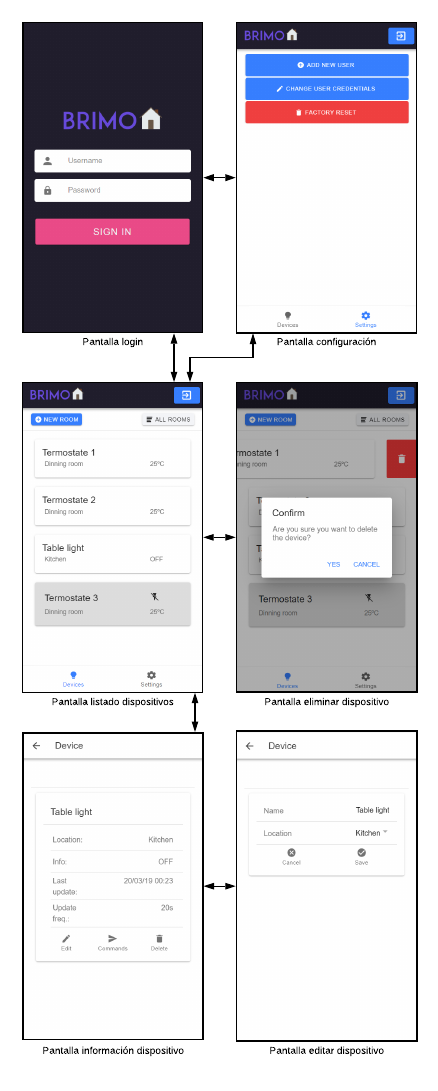
\includegraphics[width=3.50in]{images/flujo_pantallas.png}
\caption{Flujo de pantallas de la interfaz}
\label{fig:flujo_pantallas}
\end{figure}

\subsubsection{Componentes}
Para el desarrollo de la aplicación se han utilizado los siguientes UI Components de Ionic:
\begin{itemize}
\item\textbf{ion-button}: son un componente básico de la UI. Se trata de botones, pueden ser personalizados con iconos, colores, formas...etc.
\item\textbf{ion-icon}: otro componente básico de la UI. Este componente nos permite encapsular iconos en componentes ionic. Ionic ofrece una librería de
iconos bastante extensa, de la cual se han sacado todos los iconos de la aplicación: https://ionicons.com/.
\item\textbf{ion-input}: son inputs encapsulados en componentes ionic. Existen diferentes tipos de inputs: text, password, email, etc. y pueden ser customizados
de diferentes maneras. Se han utilizado, por ejemplo, en la pantalla de login, para introducir usuario y contraseña.
\item\textbf{ion-tabs}: son un componente de navegación. Cada ``tab`` corresponde a una pantalla, y navegar entre ellas a través de la barra inferior de
navegación. En nuestro caso, la aplicación contiene dos tabs: ``devices`` y ``settings``, correspondientes a las pantallas listado de dispositivos y
de configuración.
\item\textbf{ion-header}: nos permite añadir una cabecera a la pantalla. En nuestro caso, la cabecera principal (igual para todas las tabs), contiene un botón
de logout y el logo de la aplicación.
\item\textbf{ion-cards}: se trata de un componente estándar a la hora de hacer interfaces en ionic, y sirven para agrupar información por bloques. En nuestro caso,
 se utilizan cards en las pantallas de listado de dispositivos y de información/edición del dispositivo. En la pantalla de listado de dispositivos
 cada dispositivo corresponde a una ``ion-card``. Tienen subcomponentes como header, title, subtitle, content, etc.
\item\textbf{ion-list}: este componente nos permite hacer listas de otros componentes. En el caso de nuestra aplicación lo usamos en la pantalla de listado
de dispositivos, donde hacemos una lista de ``ion-cards``; y en la pantalla de configuración, donde hacemos una lista de ``ion-buttons``.
\item\textbf{ion-item-sliding}: son componentes deslizables. Se puede customizar de diferentes maneras, y añadir callbacks o componentes ocultos que aparecen
cuando el componente padre se desliza. En nuestro caso, en la pantalla de dispositivos, cada uno de ellos, a parte de ser un ion-card es un item-sliding, lo que
nos permite deslizar el dispositivo a la izquierda para que se muestre el botón de eliminar dispositivo.
\end{itemize}
\newpage
En el siguiente ejemplo se muestran los componentes utilizados en la pantalla de listado de dispositivos:
\begin{figure}[H]
\centering
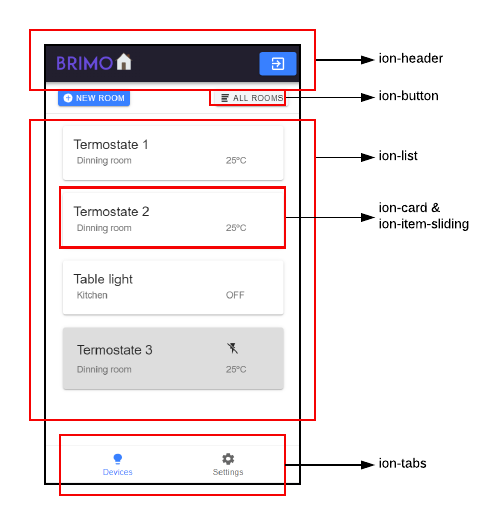
\includegraphics[width=3.50in]{images/ion_components.png}
\caption{Componentes utilizados en la pantalla listado de dispositivos}
\label{fig:ion_components}
\end{figure}

\subsection{Servicios}
Los servicios sirven para compartir funcionalidad entre los componentes. En nuestro caso, serán los encargados de comunicarse con el exterior, es decir, de hacer peticiones al HUB.
Los servicios son independientes de la interfaz, es la interfaz quien los invoca. Por ejemplo, en la pantalla de login, la interfaz se encarga de recoger los datos (usuario y
contraseña) e invocar al servicio de login, que tras hacer una petición al HUB devolverá una respuesta que será procesada de nuevo por la interfaz, mostrando un mensaje de error en
caso de fallo o navegando a la pantalla principal en caso de éxito.
\par
Para el desarrollo de nuestra aplicación hemos creado dos servicios que se encargarán de comunicarse con el HUB y un servicio para comunicar componentes entre sí:
\begin{itemize}
\item\textbf{Servicio de autenticación}: se encarga de comprobar si el usuario está logado y de recuperar el token JWT. Además, este servicio hace las llamadas de login y registrar/modificar
usuario. Cuando se hace una llamada de login el token JWT obtenido se guarda en la memoria del dispositivo, para ser recuperado cada vez que se hace una petición.
\item\textbf{Servicio de comunicación}: se encarga de comunicarse directamente con el HUB. Utiliza el servicio de autenticación para recuperar el token JWT y añadirlo en las cabeceras de 
cada petición. Este servicio sirve para añadir habitaciones, eliminar dispositivos, editar dispositivos...etc.
\item\textbf{Servicio compartido}: este servicio se encarga de comunicar componentes entre sí. Funciona con observables, a los que cada componente se suscribe en el caso de ser necesario.
Funciona, por ejemplo, para saber que el token ha caducado: si cualquier petición recibe un 401 entonces envía un evento a este servicio para que el resto de componentes (que se haya suscrito
a dicho tipo de eventos) lo sepa y la aplicación redirija automáticamente a la pantalla de login.
\end{itemize}


\chapter{Experimentos Realizados y Resultados}
\label{chap:experimentos}

\lsection{Bases de datos y protocolo}

\lsection{Sistemas de referencia}
\label{sect:sistemasreferencia}

\lsection{Escenarios de pruebas}
\label{sect:escenarios_pruebas}
 
\lsection{Experimentos del sistema completo}


\chapter{Conclusiones y trabajo futuro}
\label{chap:conclusiones}


\newpage \thispagestyle{empty} % Página vacía 

\chapter*{Glosario de acrónimos}
\addcontentsline{toc}{chapter}{Glosario de acrónimos}

\begin{itemize}
  
\item{\textbf{Sistema domótico}: Un sistema domótico es el conjunto de controladores y dispositvios que hacen posible la automatización del hogar.}
\item{\textbf{Dispositivo domótico}: Dispositivo que nos ayuda a la automatización del hogar actuando o recopilando información. Ejemplos: sensores de temperatura, relés, cámaras...etc. }
\item{\textbf{Bridge}: Dispositivo que nos ayuda a controlar y administar diferentes dispositivos domóticos. Los dispositivos se conectan al bridge, y el cliente interactua directamente a través de él. }
\item{\textbf{REST}: Arquitectura software que se apoya en el protocolo HTTP. Se utiliza en arquitecturas cliente-servidor. El cliente tiene operaciones básicas y predefinidas: GET, POST, PUT, DELETE... Y el sevidor responde a las peticiones con su correspondiente código HTTP.
Cada recurso del servidor es direccionable a través de su URI.}
\item{\textbf{Angular5}: Framework de código abierto mantenido por Google para la creación y mantenimiento de Single Page Applications (SPA). Desarrollado en TypeScript. }
\item{\textbf{SPA}: Del inglés Single Page Application: aplicación web que se ejecuta en una sola página, sin necesidad de refrescar el navegador, haciendo más fluida la navegación.}
\item{\textbf{MVC}: Modelo Vista Controlador: arquitectura software que separa los datos (Modelo) de la interfaz de usuario (Vista), su comunicación y lógica se encuentra en el controlador.}
\item{\textbf{Responsive}: Diseño web cuyo objetivo es adaptar la apariencia de la página web a diferentes dispositivos.}
\item{\textbf{Ataque Man-In-The-Middle}: Tipo de ataque en el que el atacante es capaz de interceptar y/o modificar mensajes enviados entre dos partes. 
Comúnmente este ataque se realiza en redes donde se utilizan protocolos HTTP, el atacante es capaz de captar las peticiones y modificarlas.}
\end{itemize}

\newpage \thispagestyle{empty} % Página vacía

\addcontentsline{toc}{chapter}{Bibliografa}    %Agregamos al ndice el capitulo de bibliografa 

\bibliographystyle{unsrt}   %plain pero ordenado en orden de aparacicion en documento principal
\bibliography{bibliografia}

\appendix   %Indicamos que lo que viene a continuación son apéndices

%\frontmatter %Para poner los anexos en numeros romanos

\chapter{Pantallas aplicación}
\label{Anexo:pantallas}
\begin{figure}[!htb]
\minipage{0.32\textwidth}
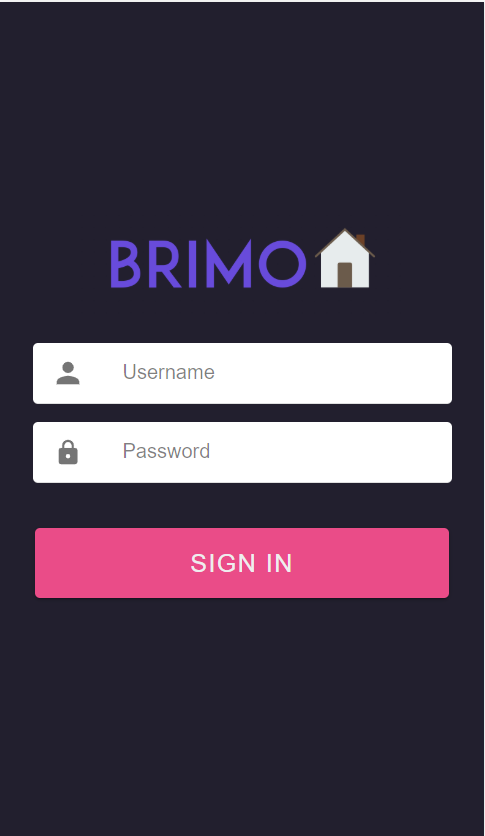
\includegraphics[width=2.00in]{images/screens/login_screen.PNG}
\caption{Pantalla de login a la aplicación}
\label{fig:pantalla_login}
\endminipage\hfill
\minipage{0.32\textwidth}
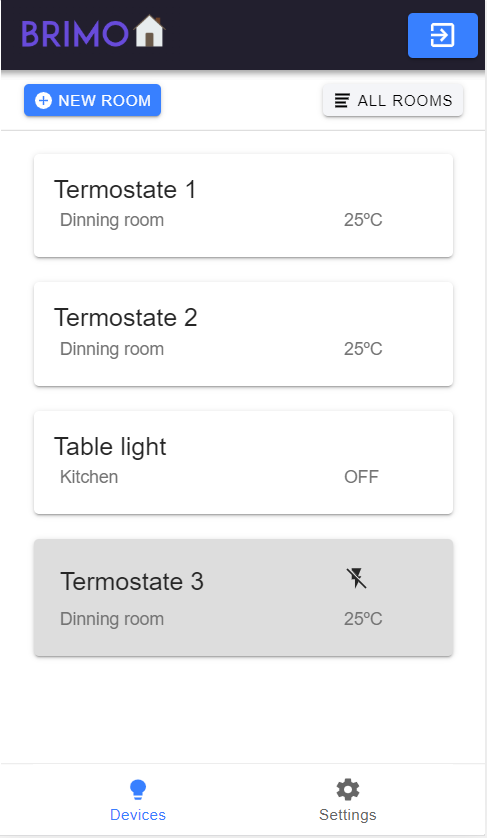
\includegraphics[width=2.00in]{images/screens/main_screen.PNG}
\caption{Pantalla listado de dispositivo}
\label{fig:pantalla_main}
\endminipage\hfill
\minipage{0.32\textwidth}%
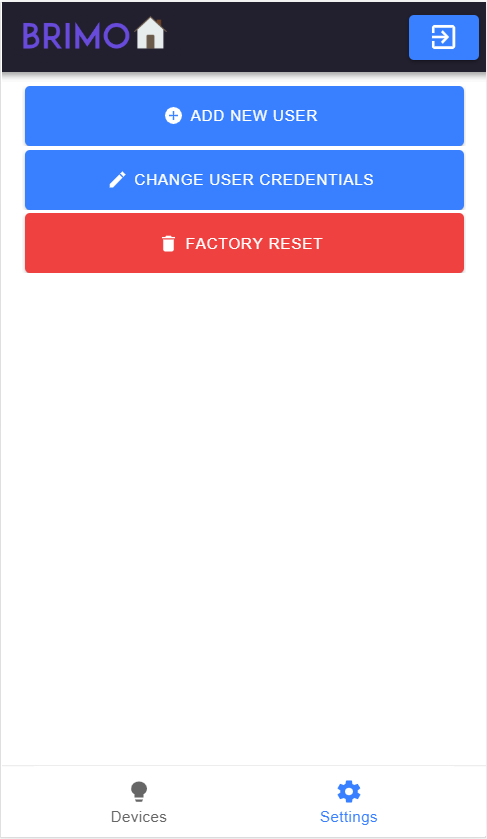
\includegraphics[width=2.00in]{images/screens/settings_screen.PNG}
\caption{Pantalla de ajustes del HUB}
\label{fig:pantalla_settings}
\endminipage
\end{figure}

\begin{figure}[!htb]
\minipage{0.32\textwidth}
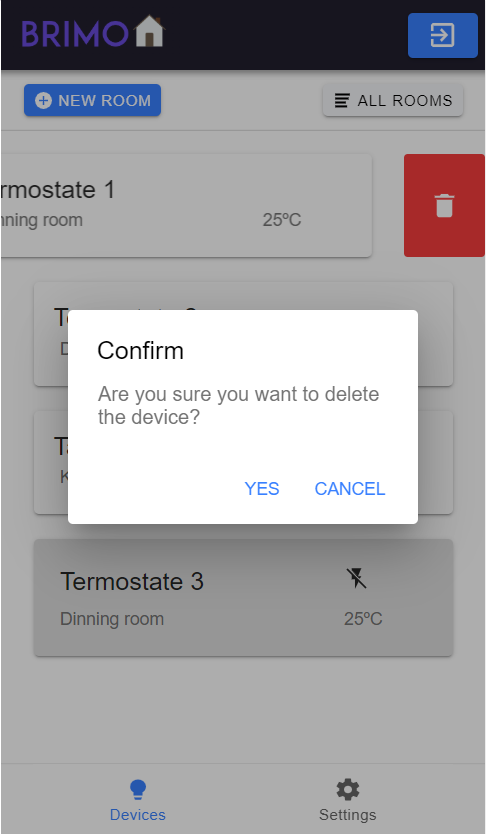
\includegraphics[width=2.00in]{images/screens/confirm_delete_screen.PNG}
\caption{Vista confirmar eliminar dispositivo}
\label{fig:pantalla_confirmar_eliminar}
\endminipage\hfill
\minipage{0.32\textwidth}
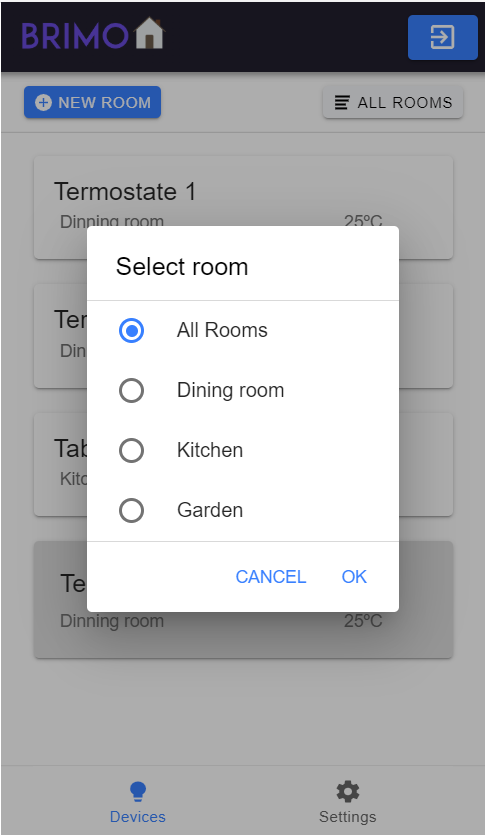
\includegraphics[width=2.00in]{images/screens/filter_screen.PNG}
\caption{Pantalla filtrar por habitación}
\label{fig:pantalla_filtrar}
\endminipage\hfill
\minipage{0.32\textwidth}%
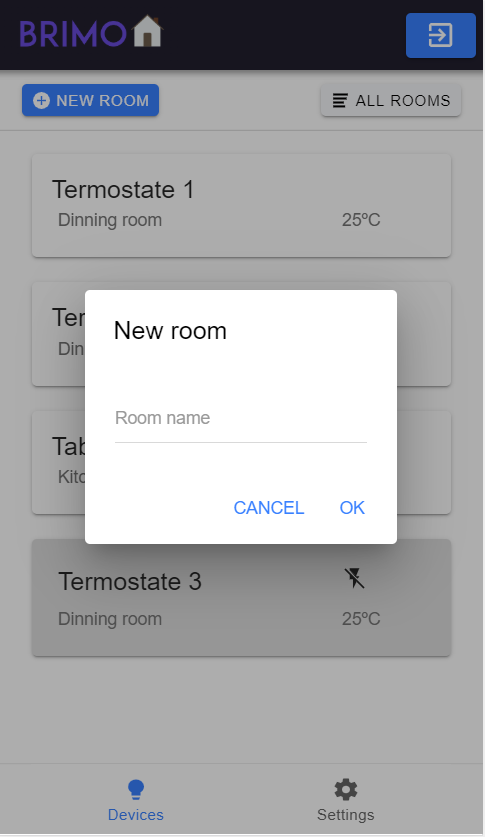
\includegraphics[width=2.00in]{images/screens/new_room.PNG}
\caption{Pantalla crear habitación}
\label{fig:pantalla_nueva_habitacion}
\endminipage
\end{figure}

\begin{figure}[!htb]
\minipage{0.32\textwidth}
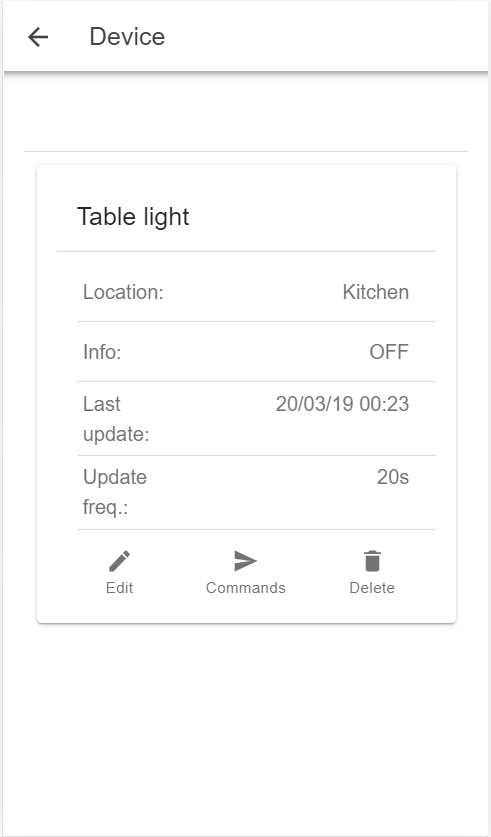
\includegraphics[width=2.00in]{images/screens/device_screen.PNG}
\caption{Vista individual dispositivo}
\label{fig:pantalla_dispositivo}
\endminipage\hfill
\minipage{0.32\textwidth}
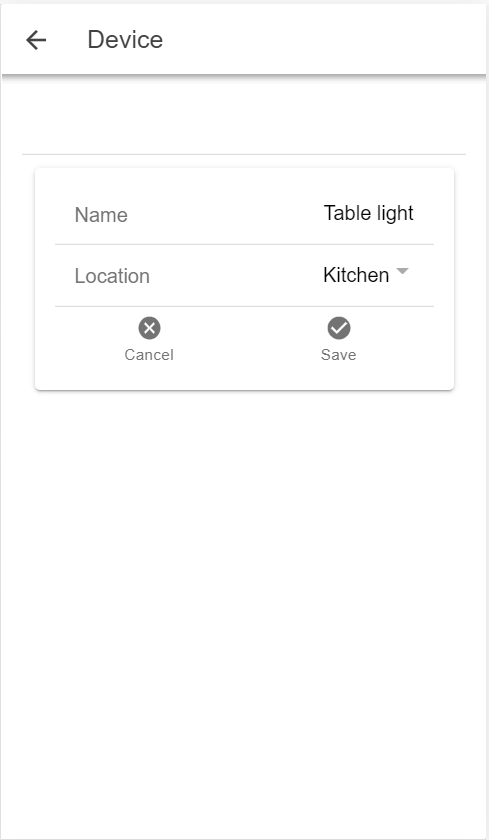
\includegraphics[width=2.00in]{images/screens/edit_device_screen.PNG}
\caption{Pantalla editar dispositivo}
\label{fig:pantalla_editar}
\endminipage\hfill
\minipage{0.32\textwidth}%
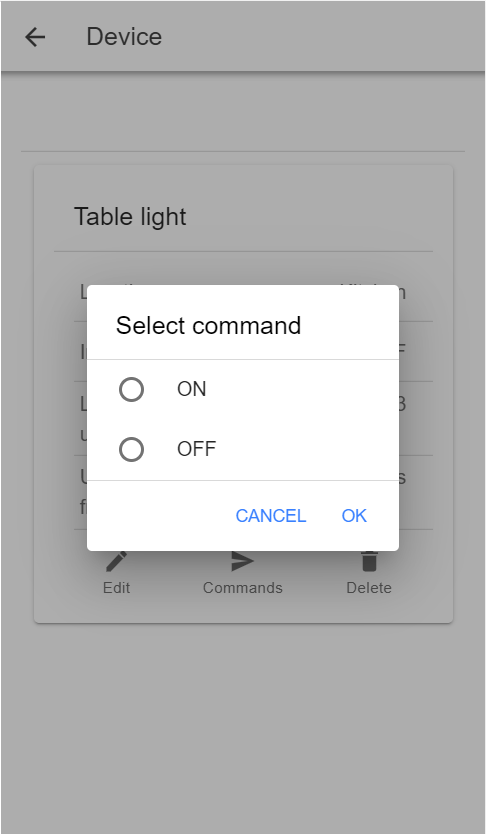
\includegraphics[width=2.00in]{images/screens/send_command.PNG}
\caption{Pantalla enviar comando}
\label{fig:pantalla_comando}
\endminipage
\end{figure}

\begin{figure}[!htb]
\minipage{0.32\textwidth}
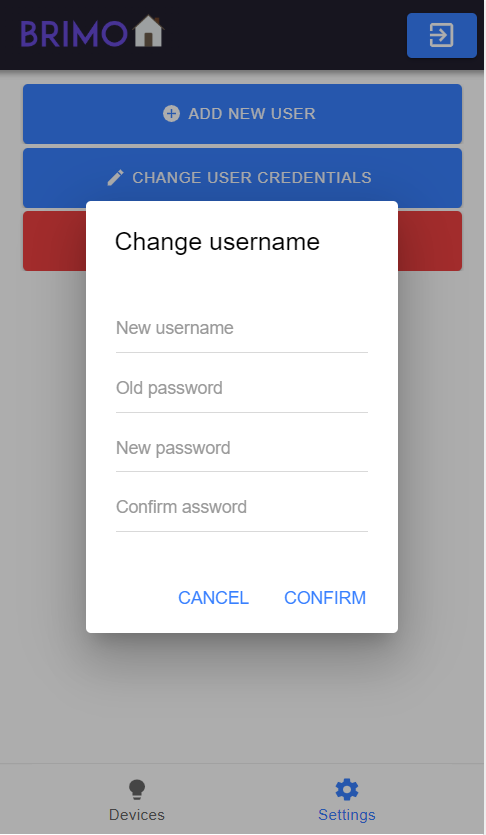
\includegraphics[width=2.00in]{images/screens/edit_username.PNG}
\caption{Diálogo editar usuario}
\label{fig:pantalla_editar_usuario}
\endminipage\hfill
\minipage{0.32\textwidth}
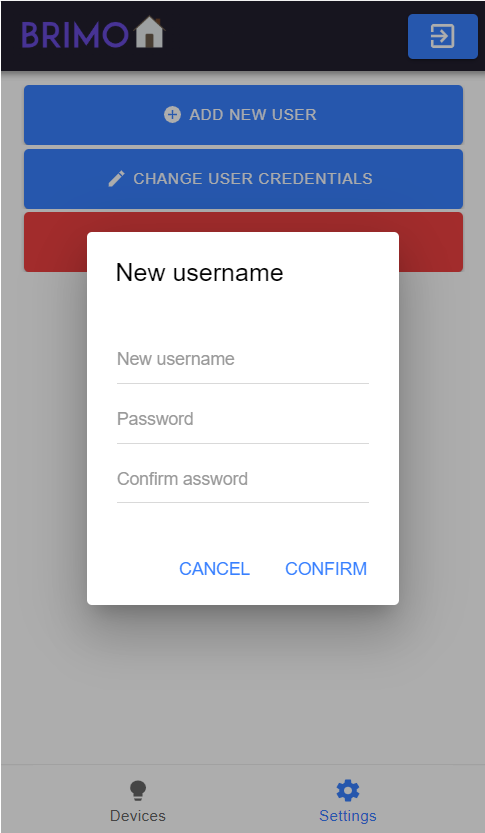
\includegraphics[width=2.00in]{images/screens/new_username.PNG}
\caption{Pantalla añadir usuario}
\label{fig:pantalla_anadir_usuario}
\endminipage\hfill
\minipage{0.32\textwidth}%
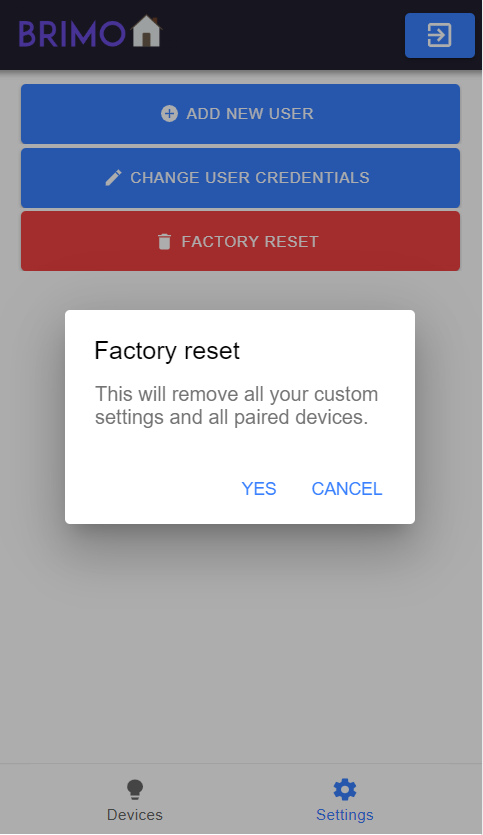
\includegraphics[width=2.00in]{images/screens/factory_reset.PNG}
\caption{Pantalla resetear HUB}
\label{fig:pantalla_factory_reset}
\endminipage
\end{figure}


\newpage \thispagestyle{empty} % Página vacía 

\chapter{Manual del programador}
\label{Anexo:codigosMatlab}


\newpage \thispagestyle{empty} % Página vacía 

%Hoja final en blanco
\newpage \thispagestyle{empty} % Página vacía

\end{document}
